% Note: This template was adapted by a report template created by Kartik Singhal under theCreative Commons Attribution 4.0 International License. You can see their template at the repository linked [here](https://github.com/googol-lab/latex-project-report-template)
% 
% View README.md for further information

\documentclass[12pt]{report}
\usepackage{amsmath}
\usepackage{amssymb}
\usepackage[pdftex]{graphicx} %for embedding images
\usepackage{url} %for proper url entries
\usepackage{appendix} %for appendix functionality
\usepackage[bookmarks, colorlinks=false, pdfborder={0 0 0}, pdftitle={}, pdfauthor={}, pdfsubject={<subject here>}, pdfkeywords={<keywords here>}]{hyperref} %for creating links in the pdf version and other additional pdf attributes, no effect on the printed document
\hypersetup{
    colorlinks=true,
    linkcolor=black,
    urlcolor=blue,
}

\usepackage{xcolor}
\usepackage{soul}
\usepackage{pdflscape} % Allow to change a page to landscape 

% BEGIN C LISTING SUPPORT
\usepackage{xcolor}
\usepackage{listings}

\definecolor{mGreen}{rgb}{0,0.6,0}
\definecolor{mBlue}{rgb}{0,0,255}
\definecolor{mGray}{rgb}{0.5,0.5,0.5}
\definecolor{mPurple}{rgb}{0.58,0,0.82}
\definecolor{MyDarkGreen}{rgb}{0.0,0.4,0.0}
\definecolor{backgroundColour}{rgb}{0.95,0.95,0.92}


\lstdefinestyle{CStyle}{
    % backgroundcolor=\color{backgroundColour},   
    commentstyle=\color{mGreen},
    keywordstyle=\color{magenta},
    numberstyle=\tiny\color{mGray},
    stringstyle=\color{mPurple},
    basicstyle=\footnotesize\ttfamily,
    breakatwhitespace=false,         
    breaklines=true,                 
    captionpos=b,                    
    keepspaces=true,                 
    numbers=left,                    
    numbersep=5pt,                  
    showspaces=false,                
    showstringspaces=false,
    showtabs=false,                  
    tabsize=2,
    language=C,
    postbreak=\mbox{\textcolor{red}{$\hookrightarrow$}\space},
}

\usepackage{geometry} % Widen margins for code listings
\newgeometry{left = 1in, right = 1in, top = 1in, bottom = 1in}
% END C LISTING SUPPORT

\usepackage{titlesec}
\titleformat{\chapter}[block]
  {\normalfont\huge\bfseries}{\thechapter}{20pt}{\Huge} % Formats chapters so number and chapter name are inline, comment out to revert to default  

% MATLAB 
% LaTeX settings for MATLAB code listings
% based on Ted Pavlic's settings in http://links.tedpavlic.com/ascii/homework_new_tex.ascii
\usepackage{listings}
% \usepackage[usenames,dvipsnames]{color}

% This is the color used for MATLAB comments below
\definecolor{MyDarkGreen}{rgb}{0.0,0.4,0.0}

% For faster processing, load Matlab syntax for listings
\lstloadlanguages{Matlab}%
\lstset{language=Matlab,                        % Use MATLAB
        frame=single,                           % Single frame around code
        basicstyle=\small\ttfamily,             % Use small true type font
        keywordstyle=[1]\color{mBlue}\bfseries,        % MATLAB functions bold and blue
        keywordstyle=[2]\color{mPurple},         % MATLAB function arguments purple
        keywordstyle=[3]\color{mBlue}\underbar,  % User functions underlined and blue
        identifierstyle=,                       % Nothing special about identifiers
                                                % Comments small dark green courier
        commentstyle=\usefont{T1}{pcr}{m}{sl}\color{MyDarkGreen}\small,
        stringstyle=\color{mPurple},             % Strings are purple
        showstringspaces=false,                 % Don't put marks in string spaces
        tabsize=5,                              % 5 spaces per tab
        %
        %%% Put standard MATLAB functions not included in the default
        %%% language here
        morekeywords={xlim,ylim,var,alpha,factorial,poissrnd,normpdf,normcdf},
        %
        %%% Put MATLAB function parameters here
        morekeywords=[2]{on, off, interp},
        %
        %%% Put user defined functions here
        morekeywords=[3]{FindESS, homework_example},
        %
        morecomment=[l][\color{mBlue}]{...},     % Line continuation (...) like blue comment
        numbers=left,                           % Line numbers on left
        firstnumber=1,                          % Line numbers start with line 1
        numberstyle=\tiny\color{mBlue},          % Line numbers are blue
        stepnumber=1                            % Line numbers go in steps of 1
        }

% Includes a MATLAB script.
% The first parameter is the label, which also is the name of the script
%   without the .m.
% The second parameter is the optional caption.
\newcommand{\matlabscript}[2]
  {\begin{itemize}\item[]\lstinputlisting[caption=#2,label=#1]{./MATLAB/#1.m}\end{itemize}}

% End MATLAB


\begin{document}
\renewcommand\bibname{References} %Renames "Bibliography" to "References" on ref page

%include other pages
\begin{titlepage}

\begin{center}

\textup{\small {\bf CIS 350 - 01} \\ Intro to Software Engineering }\\[0.2in]

% Title
\Large \textbf {Project Release - Security System}\\[0.5in]

% Submitted by
\normalsize Submitted by \\
Katherine Abernathy, Wade Callahan, Brendan Coffman, Hector Garcia, \& Isaiah Hendrick\\

\vspace{.3in}
Instructed by\\
{\textbf{Dr. Byron Devries}}\\[0.2in]

\vfill

% Bottom of the page
\Large{Padnos College of Engineering and Computing}\\
\normalsize
\textsc{Grand Valley State University}\\
% Grand Rapids, Michigan \\
% \vspace{0.1cm}
June 2, 2023

\end{center}

\end{titlepage}

\pagenumbering{roman} %numbering before main content starts
\listoffigures

\newpage
\pagenumbering{arabic} %reset numbering to normal for the main content
\chapter{Project Information}
Safe and secure home entry without the hassle of keys requires the development of a deadbolt whose locking and unlocking is controlled via PIN entry. The convenience of personalized PIN numbers for all users and the possibility of control through a mobile app would make home security easy.

The objective of the product is to provide convenience without sacrificing security. The scope of the proposed solution includes a deadbolt control mechanism, a method of confirming user identity via personal identification number, and possible development of wireless connectivity to provide remote access to the lock.


\section{Features}
This project is an Internet of Things (IoT) deadbolt. Containing an LCD display, keypad, and mobile application for additional features. This will allow the user to enter the pin through the onboard keyboard or send the pin through WiFi using Message Queuing Telemetry Transport (MQTT). Allowing the user to unlock the deadbolt from anywhere in the world along with entering the pin on the device.
Since this is still in development and this is the first release the lock currently only has a standard home screen, servo control, and a mobile application to control the locking/unlocking by sending a default pin.

\section{Screenshots}
The following two images are screenshots of the system in an unlocked state and a locked state. The first image is of the system locked. The second is an image of the system unlocked. 
\begin{figure}[htb]
    \begin{center}
        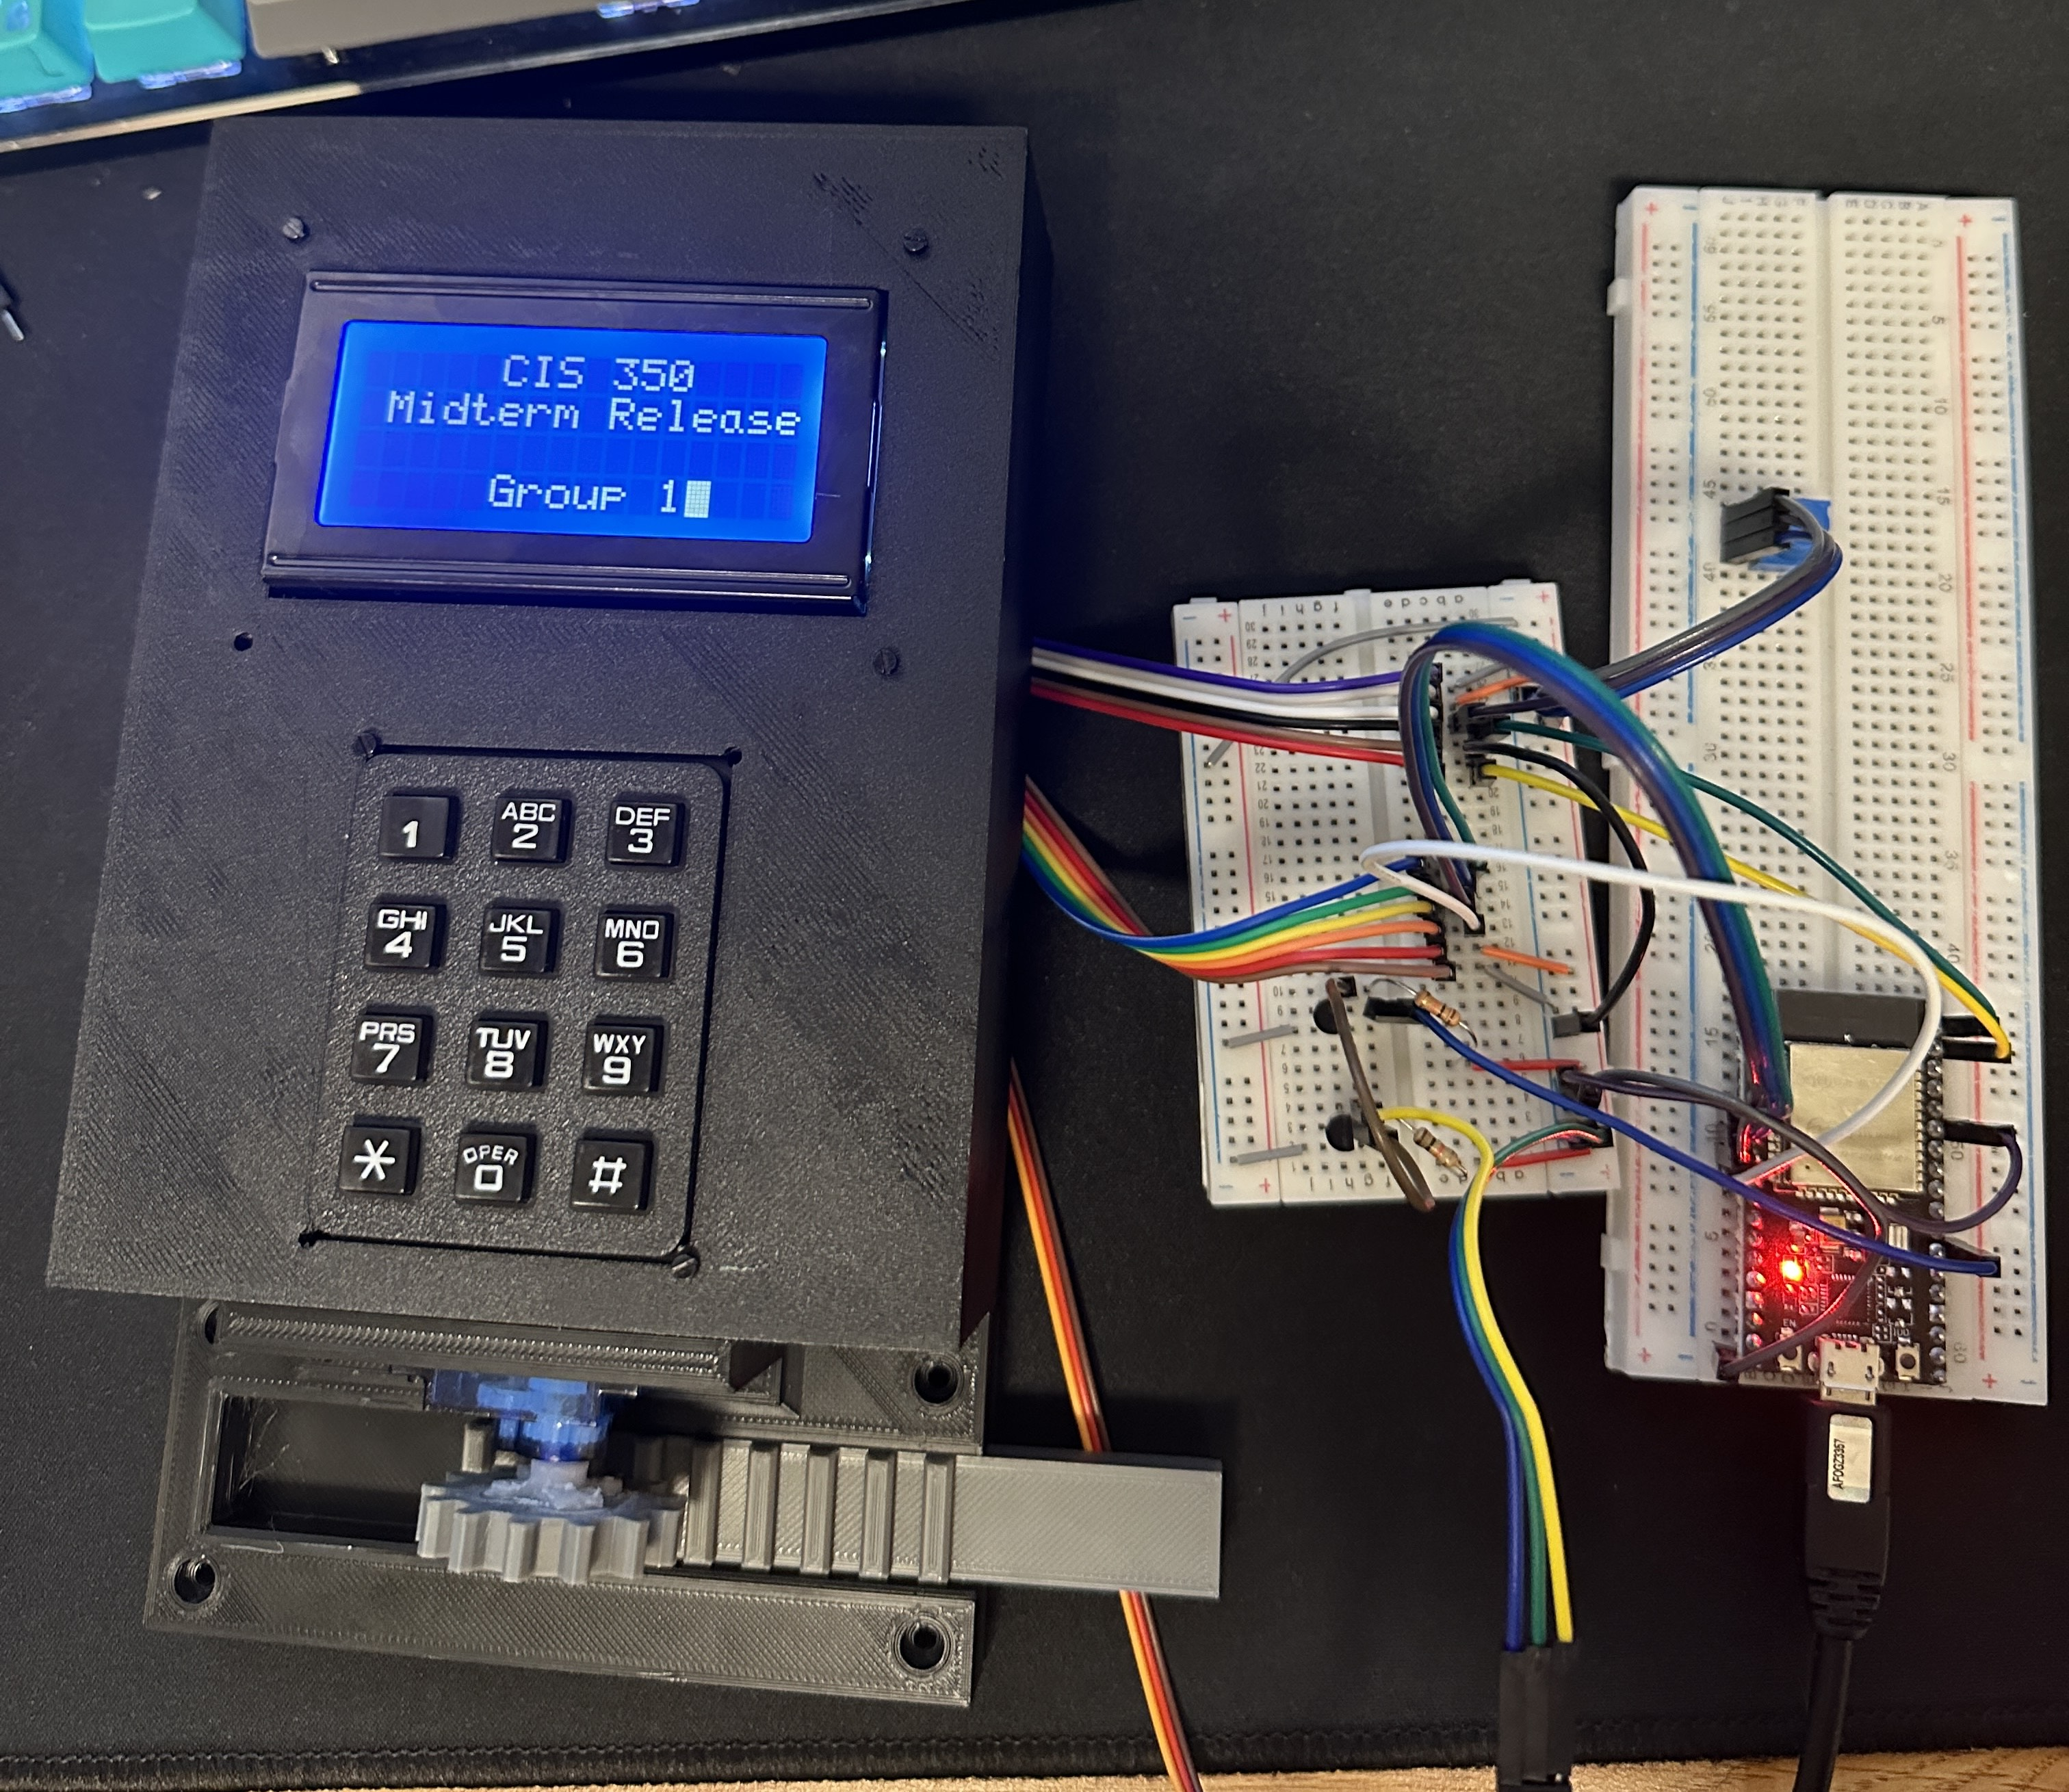
\includegraphics[width = \textwidth]{Images/Screenshot_of_system_locked.jpg}
        \caption{Image of system locked}
        \label{fig: Locked System}
    \end{center}
\end{figure}

\begin{figure}[htb]
    \begin{center}
        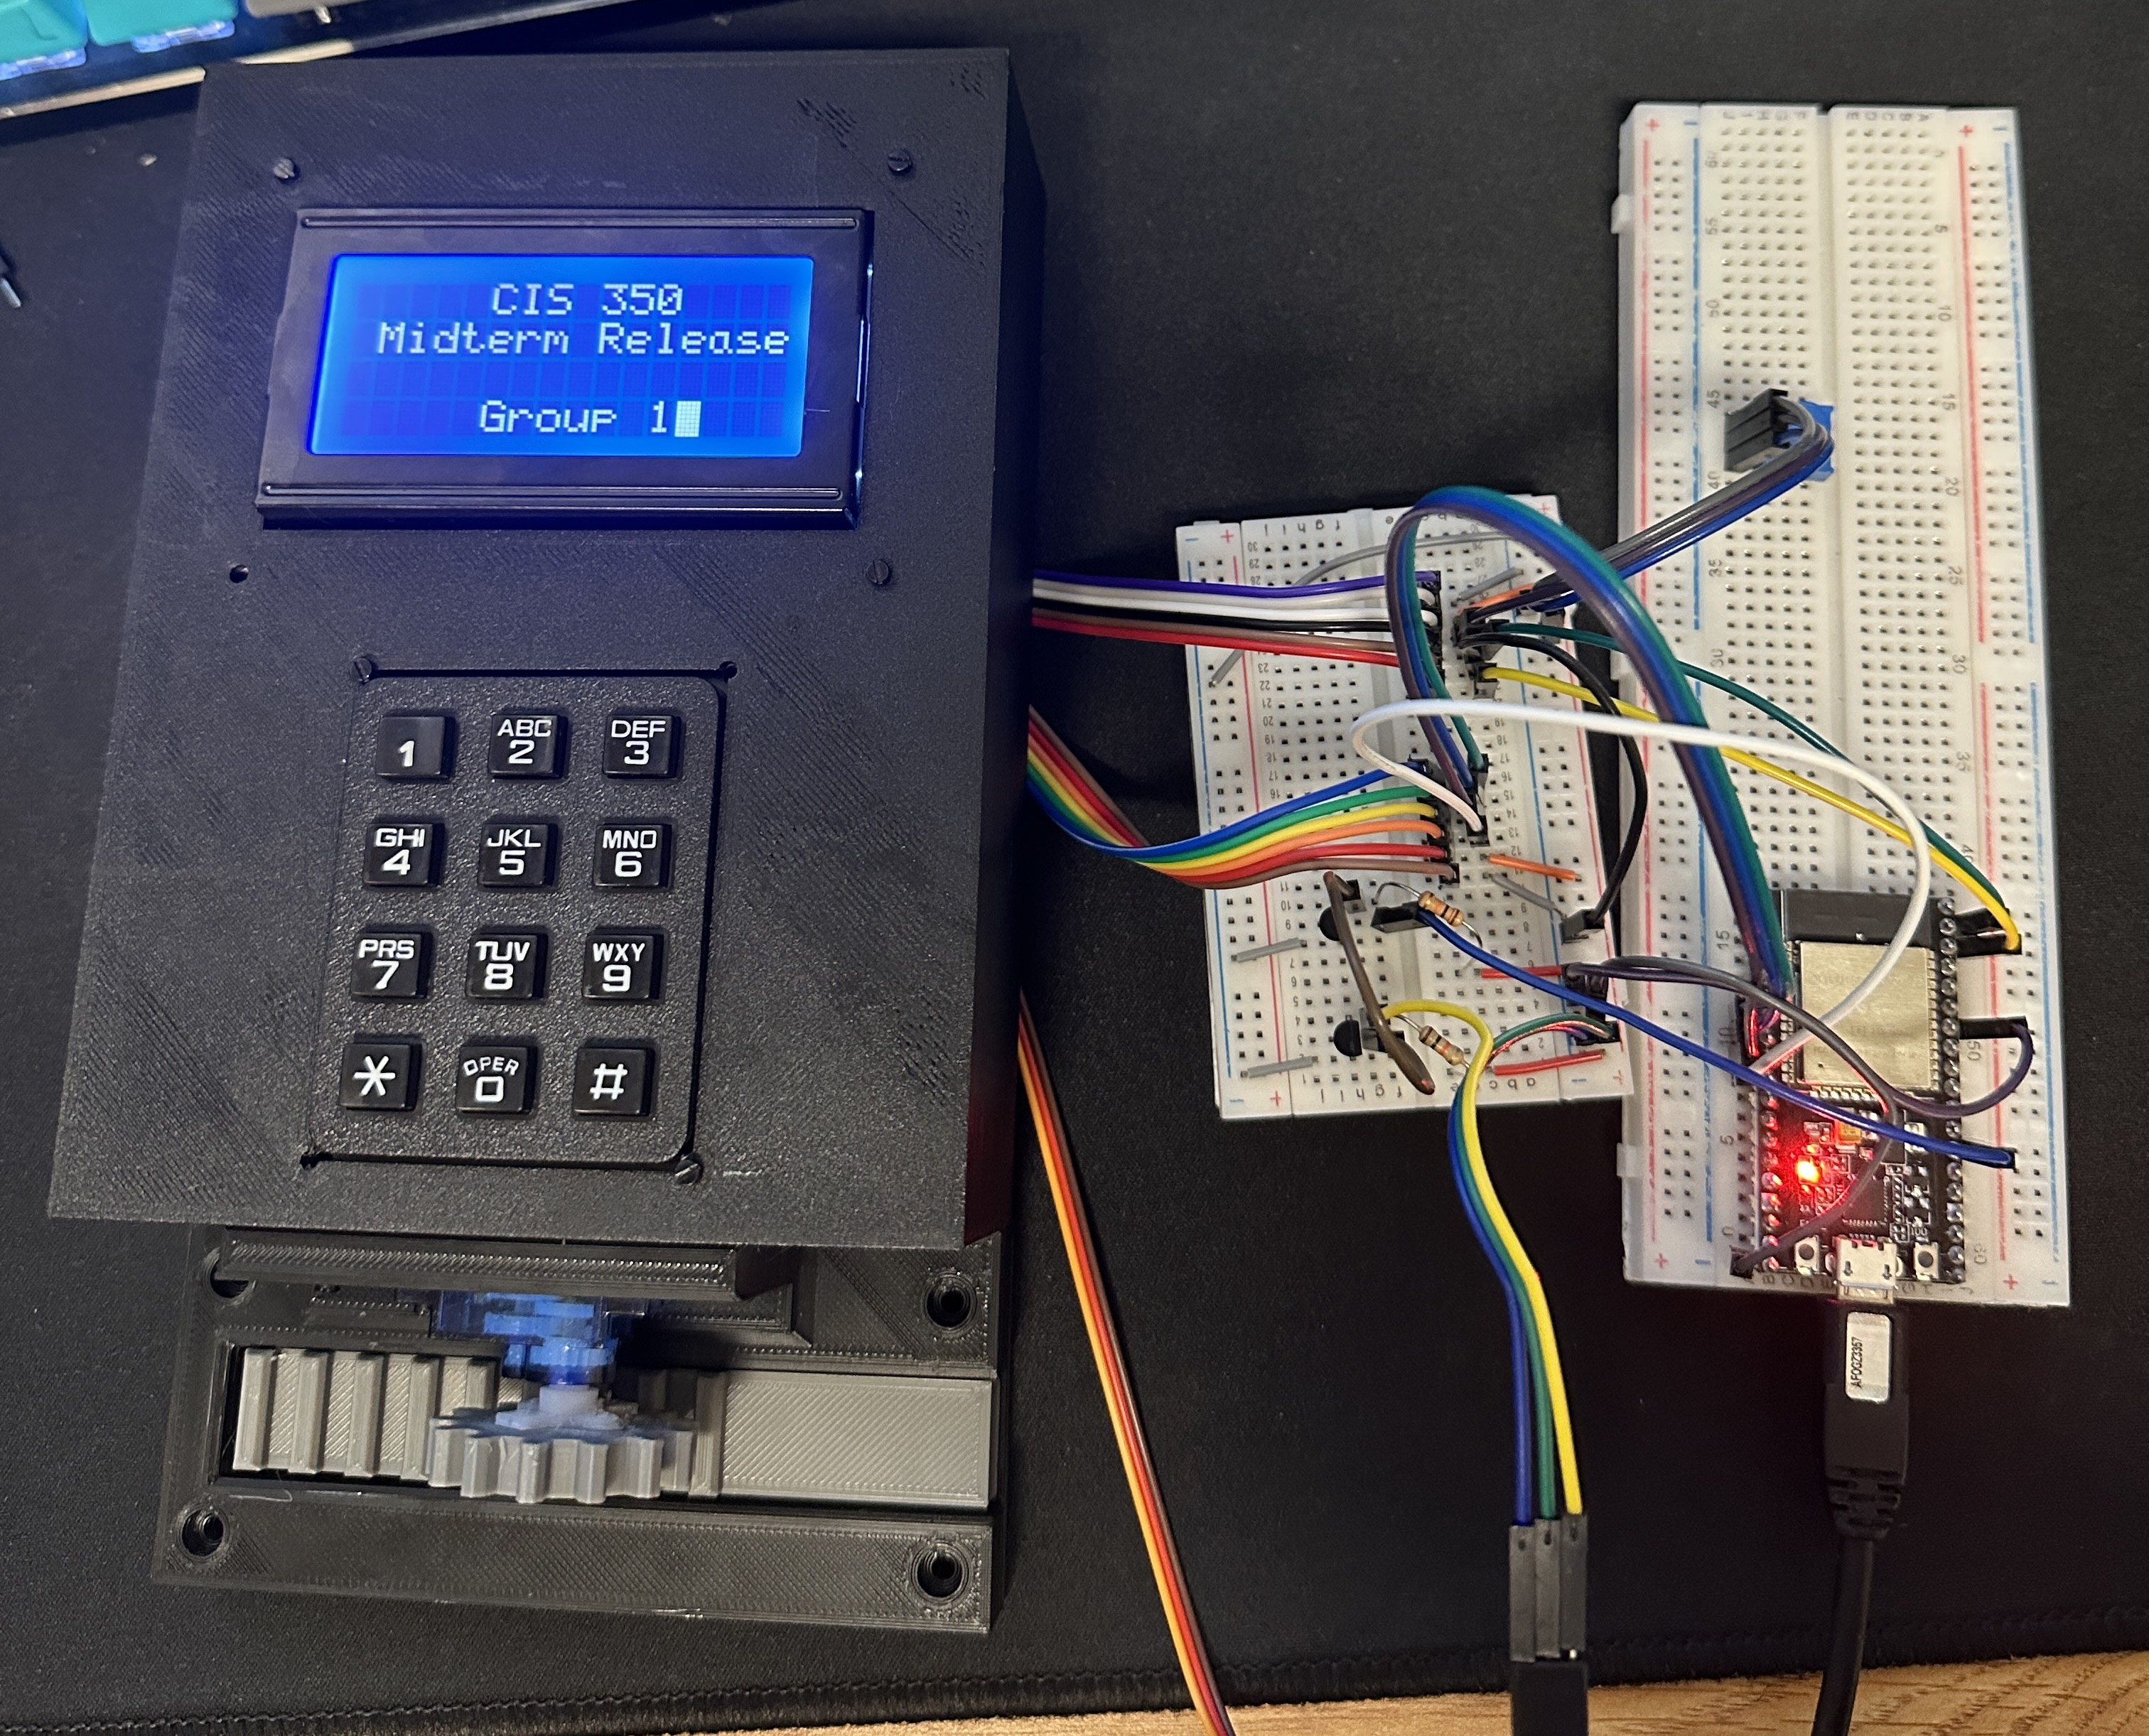
\includegraphics[width = \textwidth]{Images/Screenshot_of_system_unlocked.jpg}
        \caption{Image of system unlocked}
        \label{fig: Unlocked system}
    \end{center}
\end{figure} 
\chapter{Project Plan}
% [Overview of Project Plan, including any customizations to the software process model]

\section{Requirements \& Definition}
% [Plan for requirements and definition detailed here]
\textbf{Plan for requirement 1 and 2:} The plan is to use Message Queuing Telemetry
Transport (MQTT) to allow users to enter their pin using Wifi. \newline 

\textbf{Plan for requirement 3:} a 4 x 3 matrix keypad will be used as the external keypad. This will allow the user to enter their PIN. 

\textbf{Plan for requirement 4:} an external LCD will be configured to the ESP32 to display the numbers entered by the user. 

\textbf{Plan for requirement 5:} the system will use a function that will only store the last four (4) numbers entered by the user and validate the pass code. 

\textbf{Plan for requirement 6:} the system may have a timeout timer to determine if an input was entered, if not the external LCD will enable a screensaver. 


\textbf{Plan for requirement 7:} in the program, an integer array will store the \textit{correct} pass code. A function will be used to check if the user enters the correct pass code, the deadbolt will move to the unlock position. And, if the user enters the incorrect pass code, the deadbolt moves to the lock position. 

\textbf{Plan for requirement 8:} a state machine may be implemented, if the system is in a state that does not accept a PIN, the user will be unable to enter a PIN. A function will be used to determine the state. 

\textbf{Plan for requirement 9:} the system will use a function to determine if the entered PIN is correct or incorrect. If it is incorrect, the system will use a servo motor to control move the position of the deadbolt in the lock position. 

\textbf{Plan for requirement 10:} the system will use a function to determine if the entered PIN is correct or incorrect. If it is correct, the system will use a servo motor to control move the position of the deadbolt in the unlock position. 

\textbf{Plan for requirement 11:} the system will use a function to determine if the entered PIN is correct or incorrect. When the user enters a PIN, the LCD will use a function to display a message. 

\textbf{Plan for requirement 12:} in the program, an integer array will store multiple \textit{correct} pass codes. A function will be used to check if the user enters the correct pass code, the deadbolt will move to the unlock position. And, if the user enters the incorrect pass code, the deadbolt moves to the lock position. 

\section{Development}
% [Plan for development / implementation detailed here]
The goal for development of this project is to present a working prototype upon initial release and incorporate optional requirements as time allows. Project development thus far has followed the development of documentation required for class submission. In previous weeks, different peripherals were assigned to each group member and worked on individually. During initial release, the future states of the project were discussed. Moving forward, keypad software will be updated and the different functional parts of the project will be integrated to be demonstrated upon final release.

\section{Verification}
% [Plan for verification detailed here]
The goal for verification of the system will be mostly visual. First, when using the system upon startup, the user should see a prompt on the LCD to enter a PIN code. The user should then be able to enter numbers on the mechanical keypad located on the enclosure and see the LCD update in real time with the numbers entered. The LCD should only display up to six numbers - after that, the LCD should not print any more characters until an enter button is pressed. Upon this action, the LCD should display a "correct" or "incorrect" PIN code screen, determinant upon the code the user entered. Instead of the mechanical keypad, the user should also be able to input a PIN code from a dedicated mobile application, in which the LCD should display another "correct" or "incorrect" PIN code screen specific to the remote lock/unlock feature.

\section{Maintenance}
% [Plan for maintenance (e.g., problems found by prof or during updates for next release) detailed here] 
The goal for maintenance is to have a method to communicate issues with each other and document the solution for future reference. Within GitHub, an issue tracking feature is provided that allows developers to address and monitor bugs in the code. The process for reporting an issue includes describing the bug, detailing the expected behavior, and including any necessary screenshots or images. Once the issue is fixed, it should be marked as closed and a description of the solution should be provided. Additionally, commit messages are being used to detail each change in the software, and if a new change introduces an issue, we have the ability to quickly review past versions of the code and make the appropriate modifications.

\section{Umbrella Activities}
% [Plan for project management and status tracking / meetings detailed here]
Bi-weekly team meetings have been scheduled for the life-time of the project. These meetings are hosted via zoom and average 1.5 hours in length. During these meetings, documentation is generated and high-level project development is discussed. This time is used for collaboration on items
that need discussion as well as to ensure design and implementation agreement among members. The purpose of these meetings is to complete assignments and keep all group members on the same page. 
A google drive folder was created to share assignments with the group, allowing  for real-time collaboration. For larger documents, overleaf is utilized allowing for real-time collaboration as well. A GitHub repository was also created, allowing collaboration on source code as well as logging versions of code. Documentation was generated using the tools suggested by the professor and is included in the report.

\section{Responsibilities \& Gantt Chart}

\subsection{Responsibilities}
% [Describe the responsibilities of each member, how you plan to break down the work]
The goal for distributing the workload of this project is to spread the work based on skill set and comfort level of the assignment. However, there are certain tasks that have not been seen before by the team member or require more than one person to complete, therefore there are assignments that have more than one team member assigned. The following task were assigned to the respective team members: 

\begin{enumerate}
    \item \textbf{Mobile Application Implementation}
    \begin{itemize}
        \item Brendan Coffman 
    \end{itemize}

    \item \textbf{LCD Implementation}
    \begin{itemize}
        \item Isaiah Hendrick
        \item Hector Garcia
    \end{itemize}

    \item \textbf{Servo Implementation}
    \begin{itemize}
        \item Brendan Coffman 
    \end{itemize}

    \item \textbf{Keypad Implementation}
    \begin{itemize}
        \item Wade Callahan
        \item Katherine Abernathy
    \end{itemize}

\end{enumerate}

\subsection{Gantt Chart}
To create the project's Gantt Chart, the course project assignments, due dates, and additional tasks created by the team are gathered. As the project progresses, the chart's bars are filled to showcase the tasks that have been completed. A sample Gantt Chart is displayed on figured \ref{fig:Gantt Chart}.

\begin{figure}[htb]
    \begin{center}
        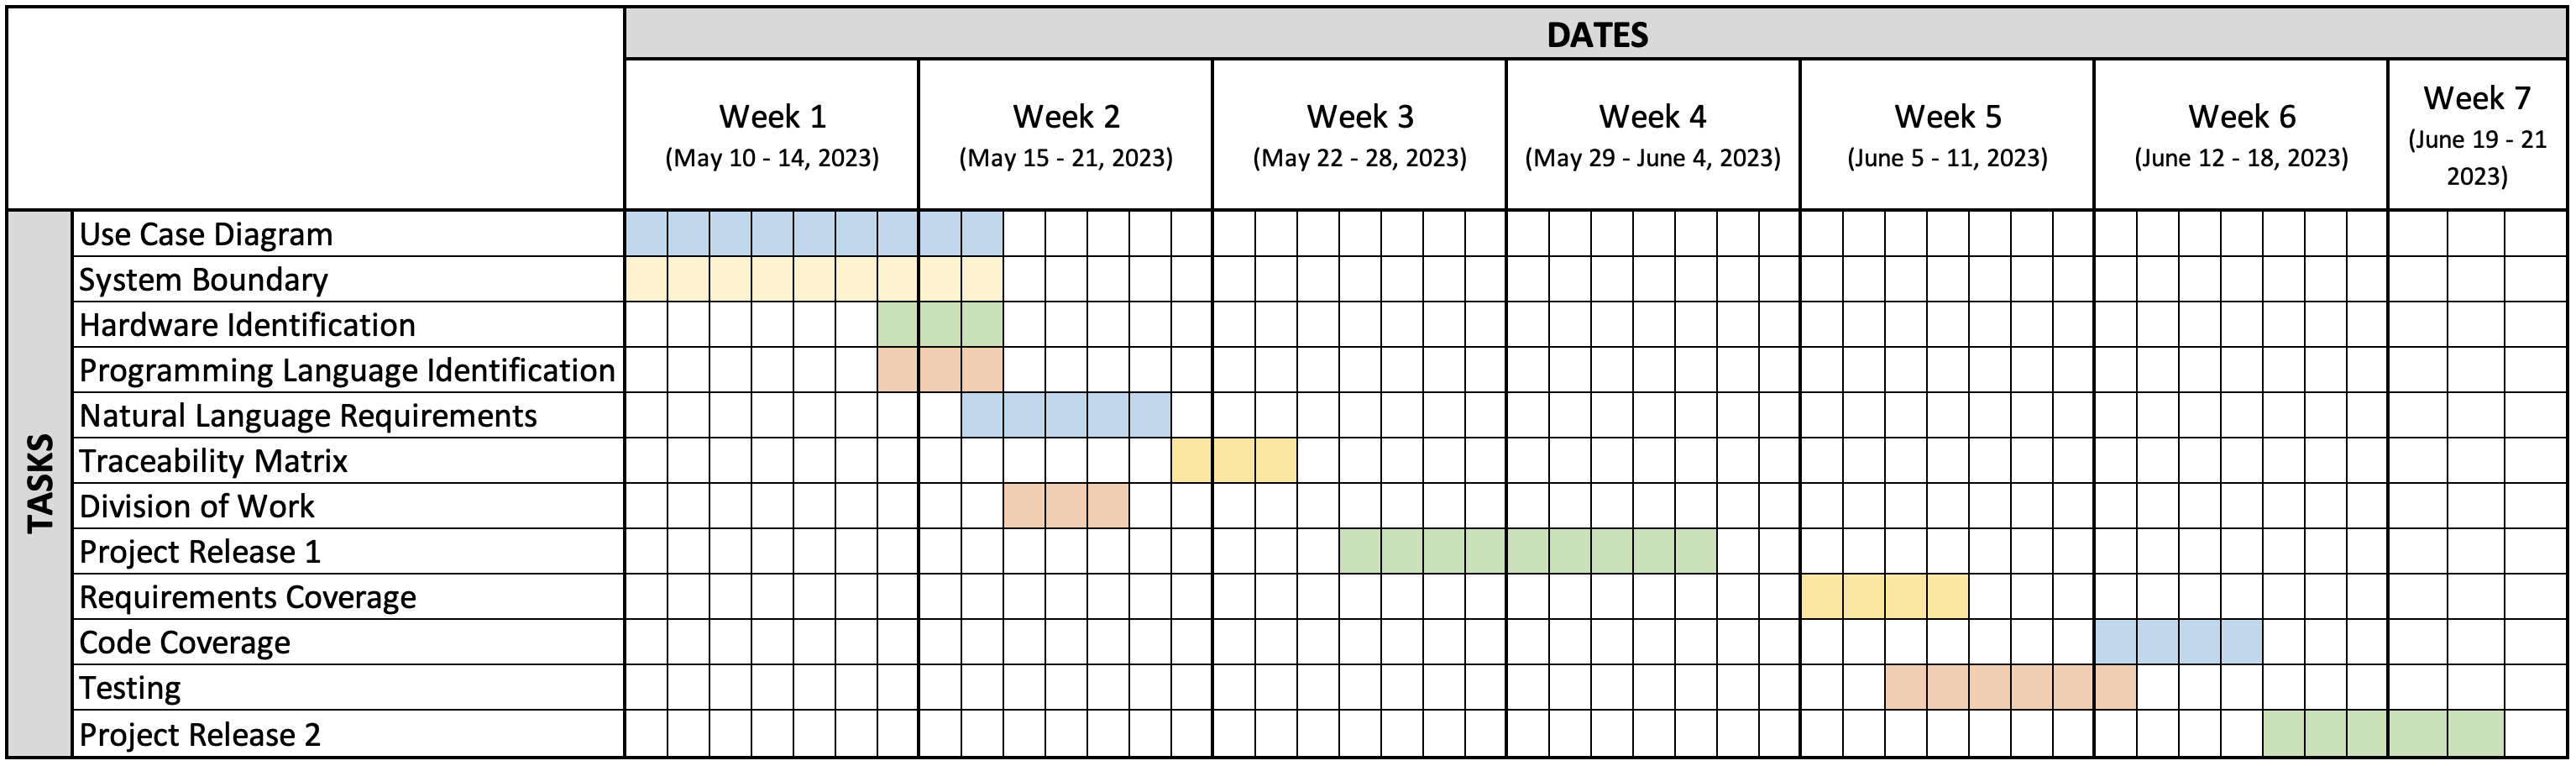
\includegraphics[width = \textwidth]{Images/CIS 350 - Project - Gantt Chart .png}
        \caption{Sample Project Gantt Chart}
        \label{fig:Gantt Chart}
    \end{center}
\end{figure}

\chapter{Requirements \& Specification}

% [Description of methods used (e.g., use- case diagrams, user stories, use case-descriptions)]

For the CIS 350 project, a use-case diagram along with use-case descriptions were used to define the actors, pre-requisites, and descriptions of the system. 

\section{Use-Cases}

\begin{figure}[htb]
    \centering
    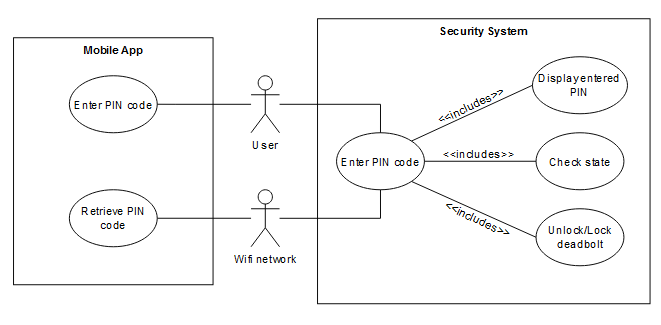
\includegraphics[width = \textwidth]{Images/CIS 350 - Project - Use Case Diagram.png}
    \caption{Project Use-case Diagram}
    \label{fig:Use-case Diagram}
\end{figure}

\newpage \textbf{Use Case Descriptions}

\begin{itemize}
    \item Security System: 
    \begin{itemize}
            \item Actors: User
            \item Pre-requisites: N/A
            \item Use Case Description: The user enters their PIN code on the keypad.
    \end{itemize}

    \item Check State: 
    \begin{itemize}
            \item Actors: User
            \item Pre-requisites: User enters a PIN
            \item Use Case Description: The current state of the lock is referenced to determine if the user has the ability to unlock vs. lock the deadbolt.
    \end{itemize}

    \item Lock/Unlock Deadbolt
    \begin{itemize}
        \item Actors: User
        \item Pre-requisites: Enter PIN and Check State
        \item Use Case Description: The servo is moved in a fashion to either unlock or lock the deadbolt based on the result of the Check State functionality referenced above. 
    \end{itemize}

    \item Display state of lock and entered PIN
    \begin{itemize}
        \item Actors: User
        \item Pre-requisites: Enter PIN
        \item Use Case Description: An LCD will display the status of the lock and if the entered PIN is incorrect. 
    \end{itemize}
    
\end{itemize}

\begin{itemize}
    \item Mobile App (Optional):
        \begin{itemize}
            \item Enter PIN Code
            \begin{itemize}
                \item Actors: User
                \item Pre-requisites: N/A
                \item Use Case Description: The user enters their PIN code on their mobile device. 
            \end{itemize}

            \item Send PIN Code
            \begin{itemize}
                \item Actors: User
                \item Pre-requisites: Enter PIN 
                \item Use Case Description: The Mobile App transmits the entered PIN code to the microcontroller wirelessly and the microcontroller determines if a PIN match has occurred.

            \end{itemize}
        \end{itemize}
\end{itemize}

\newpage \section{Natural Language Requirements}

\begin{itemize}
    \item Req 1. The security system may accept a (Personal Identification Number) PIN code from the user when using the mobile application.
    \item Req 2. The security system may retrieve PIN code from a mobile application when communicating over a Wifi network. 
    \item Req 3. The security system shall accept input from the external keypad when a button is pressed.
    \item Req 4. The security system shall display each number when the user enters them.
    \item Req 5. The security system shall display no more than the four most recently entered PIN digits when input is detected.
    \item Req 6. The security system may display a screensaver when in an idle state.
    \item Req 7. The security system shall determine when the entered code is valid after entry.
    \item Req 8. The security system may determine if a PIN code can be accepted when a key is pressed.
    \item Req 9. The security system shall lock when an invalid code is entered.
    \item Req 10. The security system shall unlock when a valid code is entered.
    \item Req 11. The security system shall display a message when a PIN code is entered.
    \item Req 12. The security system may store multiple unique PIN codes for multiple users.
    
\end{itemize}

\newpage \section{Traceability Matrix}

Table \ref{table: Traceability Matrix} - Traceability Matrix 
\begin{table}[htb]
\begin{tabular}{lccclllllllll}
                                           & \multicolumn{12}{c}{Requirement Number}                                                                                                                                                                                                                                                                      \\ \hline
\multicolumn{1}{|c|}{}                     & \multicolumn{1}{c|}{1} & \multicolumn{1}{c|}{2} & \multicolumn{1}{c|}{3} & \multicolumn{1}{l|}{4} & \multicolumn{1}{l|}{5} & \multicolumn{1}{l|}{6} & \multicolumn{1}{l|}{7} & \multicolumn{1}{l|}{8} & \multicolumn{1}{l|}{9} & \multicolumn{1}{l|}{10} & \multicolumn{1}{l|}{11} & \multicolumn{1}{l|}{12} \\ \hline
\multicolumn{1}{|l|}{Enter Pin (app)}      & \multicolumn{1}{c|}{X} & \multicolumn{1}{c|}{X} & \multicolumn{1}{c|}{}  & \multicolumn{1}{l|}{}  & \multicolumn{1}{l|}{}  & \multicolumn{1}{l|}{}  & \multicolumn{1}{l|}{}  & \multicolumn{1}{l|}{}  & \multicolumn{1}{l|}{}  & \multicolumn{1}{l|}{}   & \multicolumn{1}{l|}{}   & \multicolumn{1}{l|}{X}  \\ \hline
\multicolumn{1}{|l|}{Retrieve Pin Code}    & \multicolumn{1}{c|}{}  & \multicolumn{1}{c|}{X} & \multicolumn{1}{c|}{}  & \multicolumn{1}{l|}{}  & \multicolumn{1}{l|}{}  & \multicolumn{1}{l|}{}  & \multicolumn{1}{l|}{}  & \multicolumn{1}{l|}{}  & \multicolumn{1}{l|}{}  & \multicolumn{1}{l|}{}   & \multicolumn{1}{l|}{}   & \multicolumn{1}{l|}{}   \\ \hline
\multicolumn{1}{|l|}{Enter Pin (hardware)} & \multicolumn{1}{c|}{}  & \multicolumn{1}{c|}{}  & \multicolumn{1}{c|}{X} & \multicolumn{1}{l|}{X} & \multicolumn{1}{l|}{X} & \multicolumn{1}{l|}{}  & \multicolumn{1}{l|}{X} & \multicolumn{1}{l|}{}  & \multicolumn{1}{l|}{}  & \multicolumn{1}{l|}{}   & \multicolumn{1}{l|}{}   & \multicolumn{1}{l|}{X}  \\ \hline
\multicolumn{1}{|l|}{Pin Displayed on LCD} & \multicolumn{1}{l|}{}  & \multicolumn{1}{l|}{}  & \multicolumn{1}{l|}{}  & \multicolumn{1}{l|}{X} & \multicolumn{1}{l|}{X} & \multicolumn{1}{l|}{X} & \multicolumn{1}{l|}{}  & \multicolumn{1}{l|}{}  & \multicolumn{1}{l|}{}  & \multicolumn{1}{l|}{}   & \multicolumn{1}{l|}{X}  & \multicolumn{1}{l|}{}   \\ \hline
\multicolumn{1}{|l|}{Check State}          & \multicolumn{1}{l|}{X} & \multicolumn{1}{l|}{X} & \multicolumn{1}{l|}{}  & \multicolumn{1}{l|}{}  & \multicolumn{1}{l|}{X} & \multicolumn{1}{l|}{}  & \multicolumn{1}{l|}{X} & \multicolumn{1}{l|}{X} & \multicolumn{1}{l|}{X} & \multicolumn{1}{l|}{X}  & \multicolumn{1}{l|}{X}  & \multicolumn{1}{l|}{X}  \\ \hline
\multicolumn{1}{|l|}{Unlock/Lock Deadbolt} & \multicolumn{1}{l|}{}  & \multicolumn{1}{l|}{}  & \multicolumn{1}{l|}{}  & \multicolumn{1}{l|}{}  & \multicolumn{1}{l|}{}  & \multicolumn{1}{l|}{}  & \multicolumn{1}{l|}{}  & \multicolumn{1}{l|}{X} & \multicolumn{1}{l|}{X} & \multicolumn{1}{l|}{X}  & \multicolumn{1}{l|}{}   & \multicolumn{1}{l|}{X}  \\ \hline
\label{table: Traceability Matrix}
\end{tabular}
\end{table}
\chapter{Design}
Previous to any finite design decisions, Use Case Diagrams and System Boundaries were created in Week 1. The design of the smart lock involved important decisions about hardware and software alike. These decisions were made in the hardware identification task of our project and were completed by May 17th. The ESP32 was chosen as the microcontroller as it has WiFi capabilities built into the development board, making it compatible with the mobile app portion of the requirements. It also has an operating speed that is compatible with the peripherals chosen for the servo, LCD, and keypad. The keypad chosen was selected because of its durability in comparison to the traditional 12-key membrane keypad. This keypad uses the same logic as keypads used in previous classes so it is compatible with both prior knowledge and the chosen micro-controller. The servo and LCD chosen were also used in previous classes so there was familiarity with their functionality. A fixture was designed and 3D printed to house the peripherals and test their integration of them accordingly. During the Programming Language Identification task and due to the prior knowledge of the group members, the language chosen was C, using driver-level programming. The ultimate design while not finalized, has been laid out for future completion in the last two weeks of the course.
\chapter{Development}
% [Description of methods used (e.g., Checkstyle, PMD, Javadoc) AND any additional libraries that you used]

For this project, the program was written using the esp-idf. Which is an 
open-source driver library for the esp32 which is the micro-controller that is
being used for this project because of its low cost and built-in WI-FI
and MQTT capabilities.

To check the style of the code cpplint was used. This is based on the Google C++ style guide. 
To check for static analysis errors CppCheck was used. To generate documentation Doxygen was used.

\section{Code Standards}
% [Include report on code standards and justification for any variances]
The following is a copy of the output from cpplint. The errors are about copyright 
information not being included in the file. This is due to there not being any 
copyright information yet on this project as it is still in development and not 
intended for release. 

The other error is not including the directory when naming
header files. This is due to the compiler finding the required files in the esp-idf
that controls the building and flashing of the program. Therefore no directories can
be included in this method.
\begin{tiny}
\begin{verbatim}
main/lock_main.c:0:  No copyright message found.  You should have a line: "Copyright [year] <CopyrightOwner>"  [legal/copyright] [5]
main/lock_main.c:8:  Include the directory when naming header files  [build/include_subdir] [4]
main/lock_main.c:9:  Include the directory when naming header files  [build/include_subdir] [4]
main/lock_main.c:10:  Include the directory when naming header files  [build/include_subdir] [4]
main/lock_main.c:11:  Include the directory when naming header files  [build/include_subdir] [4]
main/lock_main.c:12:  Include the directory when naming header files  [build/include_subdir] [4]
main/lock_main.c:13:  Include the directory when naming header files  [build/include_subdir] [4]
main/lock_main.c:14:  Include the directory when naming header files  [build/include_subdir] [4]
main/lock_main.c:15:  Include the directory when naming header files  [build/include_subdir] [4]
main/lock_main.c:27:  Include the directory when naming header files  [build/include_subdir] [4]
main/lock_main.c:28:  Include the directory when naming header files  [build/include_subdir] [4]
Done processing main/lock_main.c
Total errors found: 11
\end{verbatim}
\end{tiny}

\section{Static Analysis}
% [Include report on static analysis and justification for any variances]

\begin{figure}[htb]
    \begin{center}
        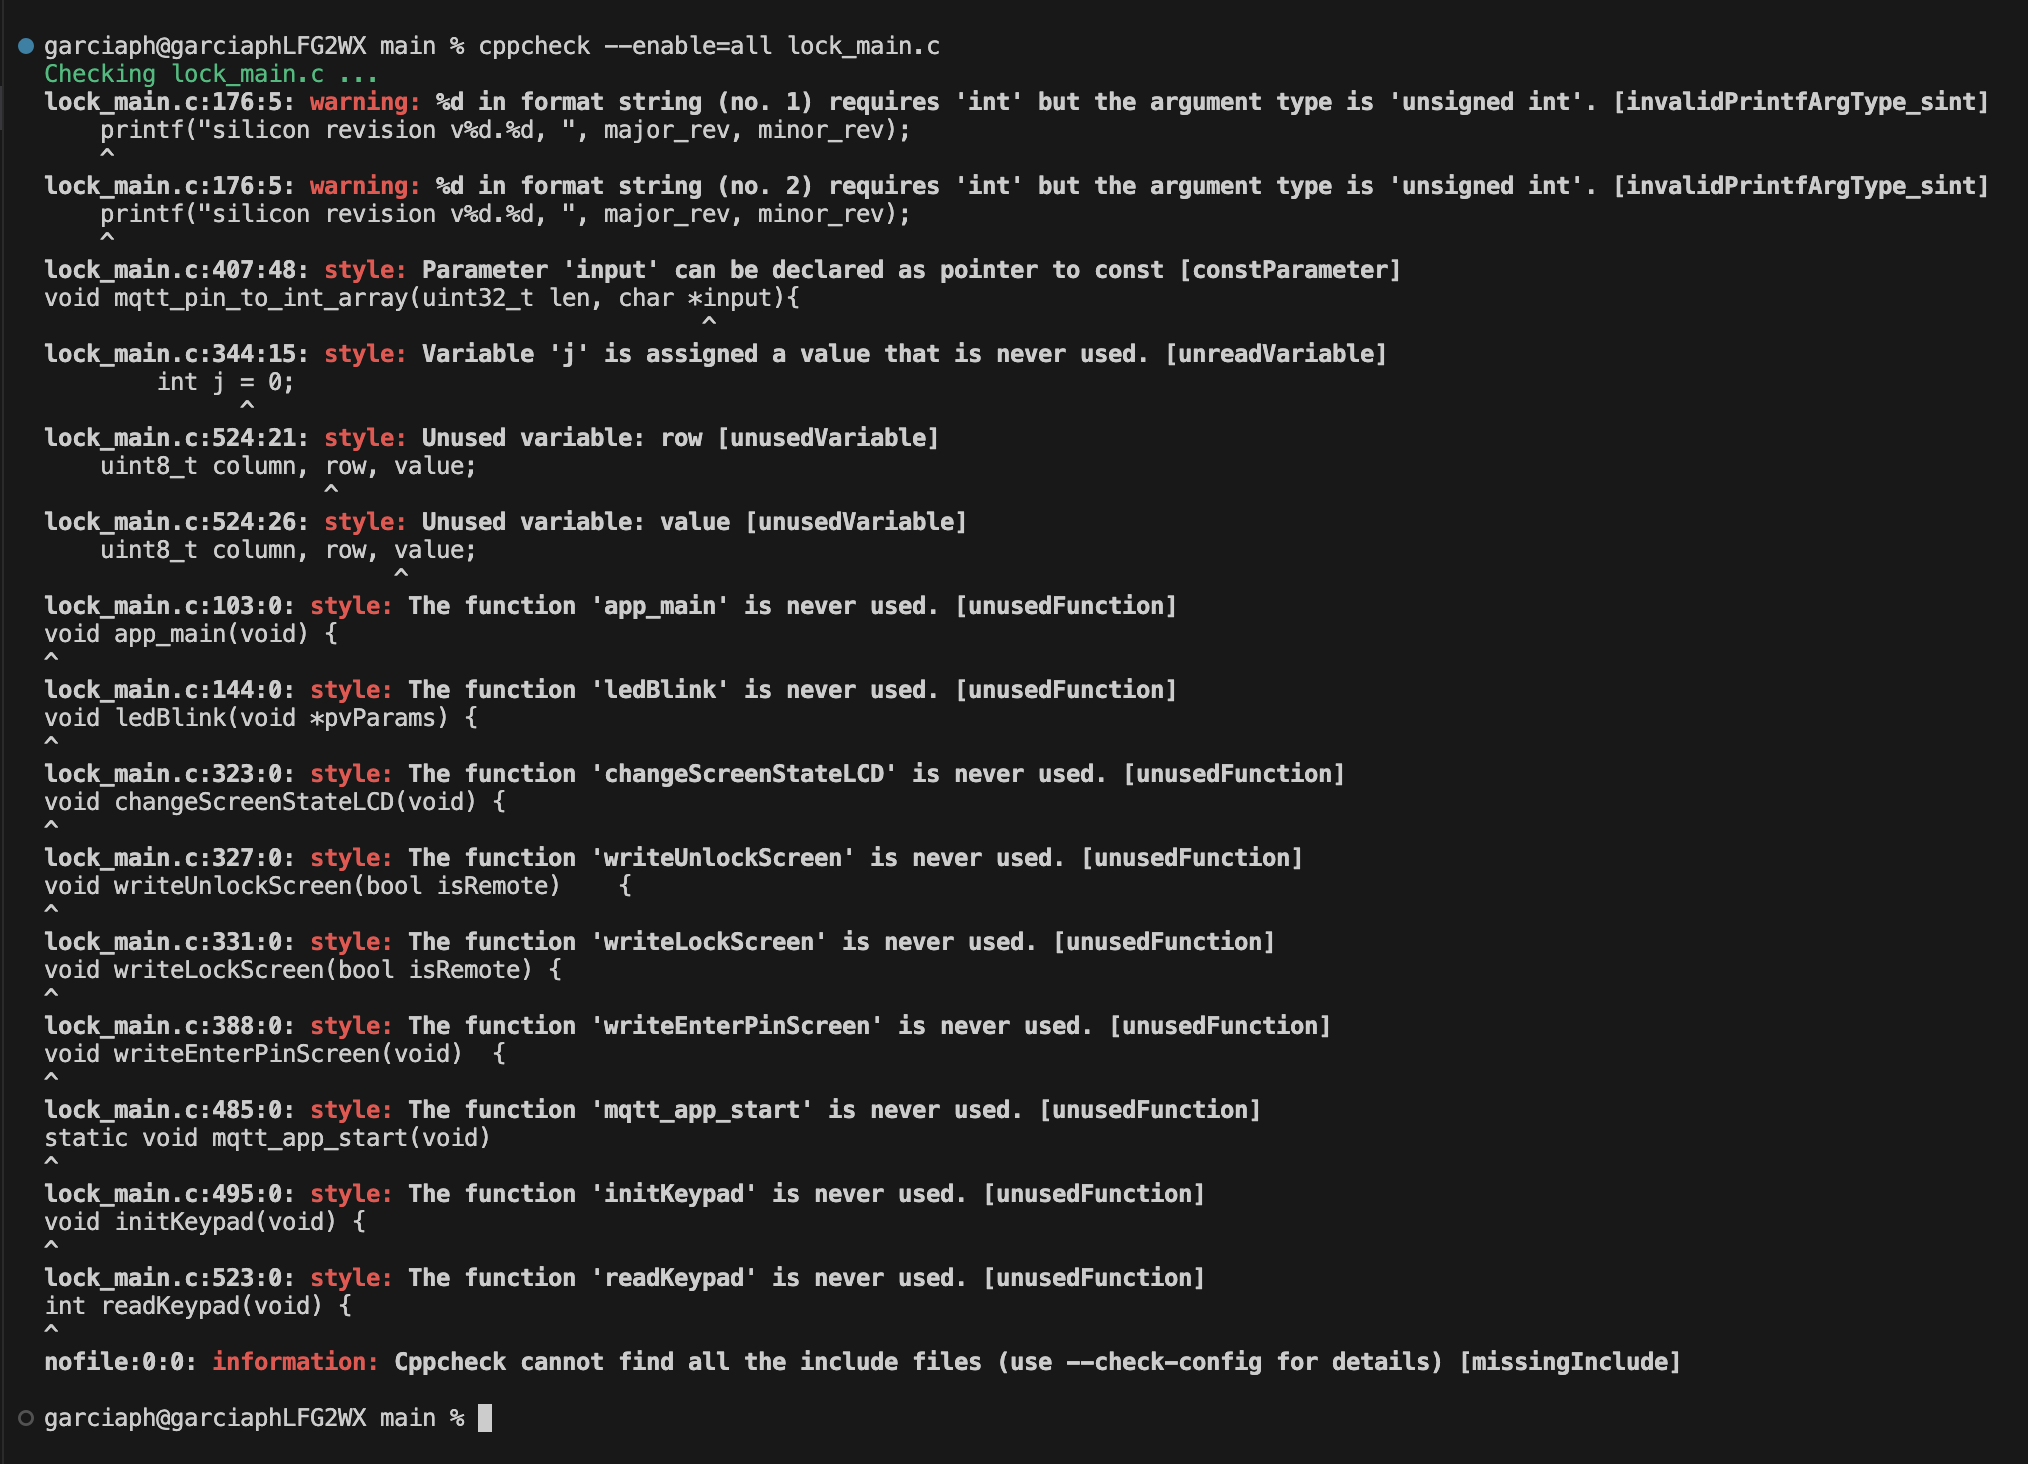
\includegraphics[width = \textwidth]{Images/CIS 350 - Project - Static Analysis Results.png}
        \caption{Static Analysis Results}
        \label{fig: Static Analysis Results}
    \end{center}
\end{figure}

The first three warnings refer to imported code that was used to verify the functionality of the selected microcontroller (MCU), ESP32. The print statements that caused the warnings will be removed. 

As for the unused function warnings, the development for some of our peripherals were started, but not completed. Once complete, the majority of the style warnings will not be reported again. 

\clearpage
\section{Code Documentation}
\subsection{Main System Documentation}
% [Include link to javadocs (likely included as separate file) and justification for any non-documented areas]
For the main system, Doxygen was used to generate the code documentation. The link to the Doxygen output is \href{https://github.com/CIS-350/lock/blob/development/html/release_1_doxygen.pdf}{here}.

\subsection{Mobile App Documentation}
For the mobile application, the project is going to be documented using DartDocs.

\section{Configuration Management}
% [Include link to Git repository and Git log] 
% [Explain / describe method for tracking releases]
The GitHub repository for the main system code base can be viewed \href{https://github.com/CIS-350/lock}{here} and the code base for the mobile lock app can be viewed \href{https://github.com/CIS-350/lock_app}{here}. In both repositories, the release specific to the midterm is labeled as "Midterm Release".\\
\\
A log containing all of the commits made to the main code base can be viewed in \hyperlink{mainlog}{\color{blue}{Appendix 8.1}} and the commits for the mobile application code base can be viewed in \hyperlink{applog}{\color{blue}{Appendix 8.2}}.\\
\\
For the project up until this point, code releases have been tracked by branching off of main for development, and merged back into main through pull requests after code development is finished. From there, a release on GitHub is created. After this midterm release however, we plan on implementing a dedicated development branch that we will be able to push changes to while still maintaining a stable code base in the main branch.

\chapter{Verification}
% [Description of methods used (e.g., integration & systems and/or unit testing)]

\section{Integration Tests}
% [Include manual and integration test procedures]
For the initial integration tests, the product will be used as instructed to ensure proper function. Then, edge cases will be identified for possible user entries and those tests will be manually performed. These tests will be designed and performed as part of the Testing task during week 5 of the project.

\section{Unit Tests}
% [Include references to unit tests in code]
Edge cases for all variables and functions used in the code will be identified and invalid inputs will be used to ensure that they are not allowed by the code. This will also be part of the Testing task during Week 5.

\section{Code Coverage}
% [Include code coverage reports, must include: coverage of automated tests, coverage of manual tests, and combined coverage]
Code Coverage will be completed during Week 5 as per the Gantt Chart.

\section{Requirements Coverage}
% [Include traceability (matrix) from requirements to test procedures]
Requirements Coverage will be completed during Week 6 as per the Gantt Chart.
\chapter{Post Mortem}
% [Include a reflection on how well the project has gone thus far]
This project has gone well so far. We are currently on schedule to complete the project before the due date and have a good amount of time for documentation. Currently, we have an MQTT connection, an LCD that we can write to, and a servo that controls the lock and unlock status of the deadbolt. The remaining features we need to implement over the next three weeks are keypad functionality and better LCD screens while the keypad is being used.
\section{Earned Value}
% [Include the earned value calculations for your current status and any explanation of over/under runs]

\section{Variances}
% [Include any additional variance (time, coverage, functionality, …) explanations necessary]
% Keypad functionality
% storing multiple pins
With this first release, the keypad functionality has not been implemented yet. Additionally, the system does not have a method to store multiple PIN codes. The LCD is also not updating as the user changes the state of the device.

\section{Lessons Learned}
% [Include lessons learned]
In the first few weeks of the project development and implementation, the following have been the lessons learned: 

\begin{enumerate}
    \item $\textbf{Project Feasibility:}$ At the beginning of the course everyone was ambitious to develop an over-the-top project. However, due to the shortened semester, the project selected was evaluated to be manageable to complete within the given time frame. 
        \begin{itemize}
            \item \textbf{Lesson Learned:} Identify a project that is realizable within the specified time frame. 
        \end{itemize}
    \item $\textbf{Assignment Delegation:}$ There are assignments that no one wants to complete or assignments no one has experience 
        \begin{itemize}
            \item \textbf{Lesson Learned:} The team members of this project are willing to lean into the unknown and learn new skills to complete the necessary assignments with high accuracy and precision. 
        \end{itemize}
    \item $\textbf{Project Management:}$ There is more to a project than programming and wiring hardware. 
        \begin{itemize}
            \item \textbf{Lesson Learned:} Proper planning and documentation is essential to a successful project. 
        \end{itemize}
    \item $\textbf{Hardware Design Issues:}$ As computer engineering students, the project has an embedded system requirement. To meet this requirement the ESP32 microcontroller was selected. As the development continued, a few issues were found with the board. Specifically that one of the ground pins was not functioning as expected.
        \begin{itemize}
            \item \textbf{Lesson Learned:} Test hardware before implementations. 
        \end{itemize}

\end{enumerate}
\cleardoublepage
%\pagebreak
\phantomsection
\addcontentsline{toc}{chapter}{References}
\begin{thebibliography}{99}

% \bibitem{citation-1-name-here}<Name of the reference here>,\ \url{<url here>}

% \bibitem{citation-2-name-here}<Name of the reference here>,\ \url{<url here>}
\bibitem{Esp-idf documentation}Esp-idf Documentation,\ \url{https://docs.espressif.com/projects/esp-idf/en/latest/esp32/}

\end{thebibliography}

\chapter{Appendix}
\section{Main System Git Log}
\hypertarget{mainlog}{}
% \addcontentsline{toc}{chapter}{Appendix}
\begin{verbatim}
commit 8d9e9033fd1be5a1d0e200a6f1b435b2e26fe29e
Merge: cd931e7 64c806b
Author: Isaiah Hendrick <hendrici@mail.gvsu.edu>
Date:   Thu Jun 1 19:53:08 2023 -0400

    Merge branch 'main' of https://github.com/CIS-350/lock

commit 64c806bc0eb2bcbfab561bc3b41e4ad0148deb25
Author: Isaiah Hendrick <107201610+hendrici@users.noreply.github.com>
Date:   Thu Jun 1 19:49:34 2023 -0400

    Update README.md

commit b87d61ba57db9cc0bc0c51f686ee87ba0b1a7dd3
Author: Isaiah Hendrick <hendrici@mail.gvsu.edu>
Date:   Thu Jun 1 19:07:34 2023 -0400

    added function comment blocks, removed ledBlink function

commit cd931e74362470691d7222426fd324d2675e9d55
Author: Isaiah Hendrick <107201610+hendrici@users.noreply.github.com>
Date:   Thu Jun 1 19:36:17 2023 -0400

    added midterm current state video to README

commit 0e55188e3aeea355b106f6210930afc0c0d93ed6
Author: Isaiah Hendrick <hendrici@mail.gvsu.edu>
Date:   Thu Jun 1 19:07:34 2023 -0400

    added function comment blocks, removed ledBlink function

commit c3b030e38ea174dd32417261131b0f7bafec3584
Author: coffmanb <coffmanb@mail.gvsu.edu>
Date:   Thu Jun 1 18:53:14 2023 -0400

    Fixed errors in linting

commit 8ac2068b66df5408ef9833989dbe208b43d6ab8c
Author: Isaiah Hendrick <hendrici@mail.gvsu.edu>
Date:   Thu Jun 1 18:16:15 2023 -0400

    added log.txt to the gitignore

commit b49ce1cd4316fff6da0818e9775a3969adf796de
Author: Isaiah Hendrick <hendrici@mail.gvsu.edu>
Date:   Thu Jun 1 18:16:03 2023 -0400

    updated text on LCD for midterm, cleaned up LCD print code

commit c33e8e9aba0492c2fa6fb79f551e50f87c5ae403
Author: Isaiah Hendrick <107201610+hendrici@users.noreply.github.com>
Date:   Wed May 31 21:17:47 2023 -0400

    Update README.md

commit 12e46c93d2003e4d25c4b4062b4b5269b55d86b7
Merge: 5651cfe 3e1e017
Author: Isaiah Hendrick <107201610+hendrici@users.noreply.github.com>
Date:   Sun May 28 22:52:17 2023 -0400

    Merge pull request \#4 from CIS-350/Isaiah-LCD
    
    added LCD functionality and code organization

commit 3e1e017b23a942d0aa3872305109d79e558025a1
Author: Isaiah Hendrick <hendrici@mail.gvsu.edu>
Date:   Sun May 28 22:49:09 2023 -0400

    made suggested changes with formatting/commenting

commit e8aa9167c4009ac290ccc8b69d6e9efa1abb977b
Author: Isaiah Hendrick <hendrici@mail.gvsu.edu>
Date:   Sun May 28 22:04:32 2023 -0400

    added LCD vars, func prototype

commit 789bc884a0bc886081b8d649a9743fec3dd65223
Author: Isaiah Hendrick <hendrici@mail.gvsu.edu>
Date:   Sun May 28 15:59:16 2023 -0400

    merged Hector's code into mine

commit 9a5b1677b319136f6cf76c2322f4ce1185f924ff
Author: Isaiah Hendrick <hendrici@mail.gvsu.edu>
Date:   Sun May 28 15:14:30 2023 -0400

    added sdkconfig.old to .gitignore

commit ba61c6fe1a65c203de2fd42d4550b3f931feee41
Author: Isaiah Hendrick <hendrici@mail.gvsu.edu>
Date:   Sun May 28 15:12:56 2023 -0400

    removed sdkconfig and sdkconfig.old, added to .gitignore

commit df4ea03ab4e3cab62d008d8a0e5a8cda650b33bb
Author: Isaiah Hendrick <hendrici@mail.gvsu.edu>
Date:   Sun May 28 15:00:15 2023 -0400

    removed .vscode from git repo

commit cbfd0fd9bfcb6af0cb4903b1425b51973f603064
Author: Isaiah Hendrick <hendrici@mail.gvsu.edu>
Date:   Sun May 28 14:55:28 2023 -0400

    added .vscode directory to .gitignore

commit 197b7d6412ec925fdeb5a1a8c99d2406220e5755
Merge: 8393bd4 5651cfe
Author: Isaiah Hendrick <hendrici@mail.gvsu.edu>
Date:   Sun May 28 14:50:19 2023 -0400

    Merge branch 'main' into Isaiah-LCD

commit 5651cfef129db878b43479da0eb5756bece5c714
Author: Brendan Coffman <112509868+coffmanb@users.noreply.github.com>
Date:   Sun May 28 14:35:31 2023 -0400

    Features/mqtt control (\#2)
    
    Control over the lock by sending pin

commit e4e244b38fe470e7c4e735a736d6c71276b7d946
Author: Brendan Coffman <112509868+coffmanb@users.noreply.github.com>
Date:   Sun May 28 14:07:00 2023 -0400

    Features/servo control (\#1)
    
    Added control of the servo via lockDeadbolt() and unlockDeadbolt() functions

commit 8393bd4aeca86261060ba23ee0b0385e48830a4a
Author: Isaiah Hendrick <hendrici@mail.gvsu.edu>
Date:   Fri May 26 16:23:40 2023 -0400

    rearrange code, LCD now working

commit 5c8723f2b57fed2680d26abafcfa82b1a58c0fb9
Author: Hector Garcia <garcihec@gmail.com>
Date:   Thu May 25 18:36:02 2023 -0400

    commented out the thread for the LED and Servo

commit a2693a252e41c915905eeb196dbac134f6322211
Author: Hector Garcia <garcihec@gmail.com>
Date:   Thu May 25 18:33:43 2023 -0400

    Added LCD commands
    
    Co-authored-by: Isaiah Hendrick <hendrici@users.noreply.github.com>

commit 5080bb2342bd3c2022ed38ceab9469f7ba2c3ed6
Author: coffmanb <coffmanb@mail.gvsu.edu>
Date:   Wed May 24 13:54:09 2023 -0400

    Latest version

commit 2865a9675d5ed6f4ad5092e9d5adb7850f5e6154
Author: coffmanb <coffmanb@mail.gvsu.edu>
Date:   Mon May 22 20:06:53 2023 -0400

    should be working code. Hardware issue

commit c1b58408bf6df789099934da8f2f066acea1c843
Author: coffmanb <coffmanb@mail.gvsu.edu>
Date:   Fri May 19 13:38:32 2023 -0400

    Potentially working code? hardware?

commit 031bea68991538e089d4c3b6c7c55f56d198cf25
Author: Hector Garcia <garcihec@gmail.com>
Date:   Thu May 18 15:59:10 2023 -0400

    made changes to README

commit 5b7d1316958079b9a9a8c190cceb3c1787f2ba40
Author: coffmanb <coffmanb@mail.gvsu.edu>
Date:   Wed May 17 18:34:26 2023 -0400

    Updated readme.md for getting started

commit 7a801a44dd1dc21f1f90ef385791c9529b320cbf
Author: coffmanb <coffmanb@mail.gvsu.edu>
Date:   Wed May 17 18:26:31 2023 -0400

    added build folder to ignored

commit 3e376698fff9dc5b12a0bea268255b91757c2e73
Author: coffmanb <112509868+coffmanb@users.noreply.github.com>
Date:   Wed May 17 18:14:59 2023 -0400

    windows build

commit 977d64f6f4613195c5babebee5b5309479f894ef
Author: coffmanb <112509868+coffmanb@users.noreply.github.com>
Date:   Tue May 16 17:08:03 2023 -0400

    Initial?

commit 740de81332fa33bc7b7761e35d814505f05982c9
Author: coffmanb <112509868+coffmanb@users.noreply.github.com>
Date:   Tue May 16 16:46:56 2023 -0400

    testing push

commit 11ff6f086e0ed213f5cf4dd9771dcc144ef95429
Author: coffmanb <112509868+coffmanb@users.noreply.github.com>
Date:   Tue May 16 16:29:59 2023 -0400

    Changed main file name

commit 30f997e1992237f1684a0f46a963a5d574901f8e
Author: coffmanb <112509868+coffmanb@users.noreply.github.com>
Date:   Sun May 14 16:31:00 2023 -0400

    Init

\end{verbatim}

\section{Mobile Application Git Log}
\hypertarget{applog}{}
\begin{verbatim}
commit 8a37e894220dc8d9c6ee1cd500c147ea41be7eaf
Author: Isaiah Hendrick <hendrici@mail.gvsu.edu>
Date:   Thu Jun 1 20:07:28 2023 -0400

    added log.txt to gitignore

commit 3a7829875c81b1fa96a0b2c4ccf52bda2d6e5b1f
Author: coffmanb <112509868+coffmanb@users.noreply.github.com>
Date:   Fri May 26 16:14:43 2023 -0400

    Updated icon better

commit c2c5a50339c763cf622a81888134b2d670014909
Author: coffmanb <112509868+coffmanb@users.noreply.github.com>
Date:   Fri May 26 16:05:56 2023 -0400

    Added an icon

commit d03c0dcf05183471367540020e62c47cd4d870d1
Author: coffmanb <112509868+coffmanb@users.noreply.github.com>
Date:   Fri May 26 15:18:19 2023 -0400

    Working communication with lock

commit 0fef0ed4d8ad77f37b5ed5928017936bf4fdf08d
Author: coffmanb <112509868+coffmanb@users.noreply.github.com>
Date:   Sat May 13 15:25:31 2023 -0400

    initial

\end{verbatim}

\end{document}